\documentclass{beamer}
\usepackage{listings}
\lstset{
%language=C,
frame=single, 
breaklines=true,
columns=fullflexible
}
\usepackage{blkarray}
\usepackage{subcaption}
\usepackage{url}
\usepackage{tikz}
\usepackage{tkz-euclide} % loads  TikZ and tkz-base
%\usetkzobj{all}
\usetikzlibrary{calc,math}
\usepackage{float}
\newcommand{\myvec}[1]{\ensuremath{\begin{pmatrix}#1\end{pmatrix}}}
\providecommand{\brak}[1]{\ensuremath{\left(#1\right)}}
\newcommand\norm[1]{\left\lVert#1\right\rVert}
\renewcommand{\vec}[1]{\mathbf{#1}}
\usepackage[export]{adjustbox}
\usepackage[utf8]{inputenc}
\usepackage{amsmath}
\usepackage{physics}
\usepackage{tikz}
\usetikzlibrary{automata, positioning}
\usetheme{Boadilla}
\providecommand{\pr}[1]{\ensuremath{\Pr\left(#1\right)}}

\title{Assignment 3 Presentation}
\author{Yashas Tadikamalla}
\date{AI20BTECH11027}
\begin{document}

\begin{frame}
\titlepage
\end{frame}

\begin{frame}
\frametitle{}
\begin{block}{Power of a point}
The power of a point is a real number that reflects the relative distance of a given point from a given circle. Specifically, the power $\Pi(P)$ of a point $P$ with respect to a circle $C$ with center $O$ and radius $r$ is defined by
\begin{align}
    \Pi(P)=\abs{PO}^{2}-r^{2}
    \label{eq:1}
\end{align}
\begin{itemize}
    \item $\Pi(P)>0\Leftrightarrow P$ is outside the circle
    \item $\Pi(P)=0\Leftrightarrow P$ is on the circle
    \item $\Pi(P)<0\Leftrightarrow P$ is inside the circle
\end{itemize}
For a circle $S=0$, \eqref{eq:1} boils down to,
\begin{align}
    \Pi(P)=S_{11}
    \label{eq:2}
\end{align}
\end{block}
\end{frame}

\begin{frame}
\frametitle{}
\begin{block}{}
\begin{figure}[!h]
 \centering
 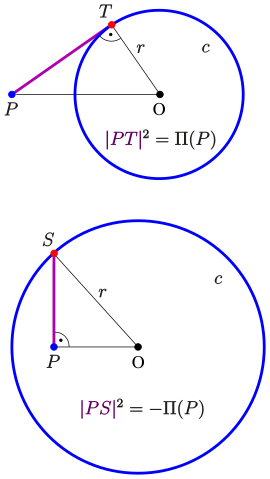
\includegraphics[width=0.25\columnwidth]{Assignment3Presentation(1).png}
 \caption{Geometric interpretation of power of a point with respect to a circle }
 \label{plot}
\end{figure}
\end{block}
\end{frame}

\begin{frame}
\frametitle{}
\begin{block}{Radical axis}
The radical axis of two non-concentric circles is the set of points whose power with respect to the circles are equal. i.e, points for which,
\begin{align}
    \Pi_{1}(P)=\Pi_{2}(P)
    \label{eq:3}
\end{align}
For two non-concentric circles $S=0,S'=0$, the radical axis is given by
\begin{align}
    L=S-S'=0
    \label{eq:4}
\end{align}
\begin{figure}[!h]
 \centering
 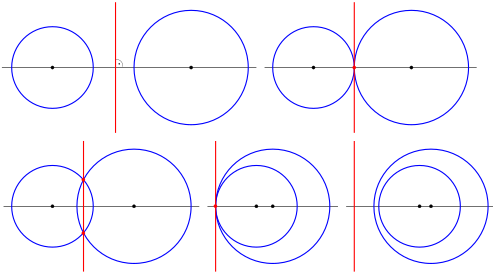
\includegraphics[width=0.4\columnwidth]{Assignment3Presentation(2).png}
 \caption{Variations of radical axis}
 \label{plot}
\end{figure}
\end{block}
\end{frame}

\begin{frame}
\frametitle{Question}
\begin{block}{Ramsey/4.4 Systems of circles/Q4 (a)}
Write down the equation of the radical axis of the following pair of circles:
$$\vec{x}^{T}\vec{x}-\myvec{
4 & -5}\vec{x}-2=0$$
$$\vec{x}^{T}\vec{x}-\myvec{
5 & -6}\vec{x}=0$$
\end{block}
\end{frame}

\begin{frame}
\frametitle{Solution}
Given, two circles with equations,
\begin{align}
S=\vec{x}^{T}\vec{x}-\myvec{4 & -5}\vec{x}-2=&0\label{eq:5}\\
S'=\vec{x}^{T}\vec{x}-\myvec{5 & -6}\vec{x}=&0\label{eq:6}
\end{align}
To find: The radical axis of the pair of circles.\\
Using \eqref{eq:4}, the required equation is
\begin{align}
\brak{\vec{x}^{T}\vec{x}-\myvec{4 & -5}\vec{x}-2}-\brak{\vec{x}^{T}\vec{x}-\myvec{5 & -6}\vec{x}=0}=&0\\
\myvec{1 & -1}\vec{x}-2=&0
\end{align}
$\therefore L=\myvec{1 & -1}\vec{x}-2=0$ is the equation of the required radical axis.
\end{frame}

\begin{frame}
\frametitle{Solution Contd.}
\begin{figure}[!h]
 \centering
 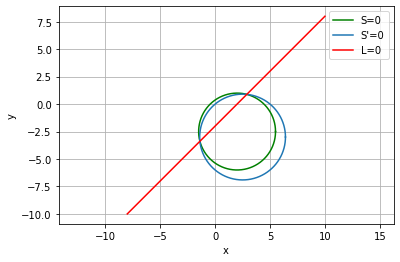
\includegraphics[width=0.75\columnwidth]{Assignment3Presentation(3).png}
 \caption{Pair of Circles and their radical axis}
 \label{plot}
\end{figure}
\end{frame}
\end{document}